\section{Brownie Point Nominations}

\begin{frame}{Brownie Point Nominations}
	Security Analysis for Skinny Cipher are based on related-key model.
	\begin{block}{Security Analysis}
		
		\begin{itemize}[<+->]
			\item Integral Attacks
			\item Meet-In-The-Middle Attacks
			\item Impossible Differential Attacks
			\item  Differential/Linear Cryptanalysis
			\item Slide Attacks
		\end{itemize}
	\end{block}
\end{frame}


\begin{frame}{Integral Attacks}
	
	\begin{itemize}[<+>]
		\item Cell size can be 4 or 8 bits.
		\item All(A)
		\item Balance(B)
		\item Constant(C)
		\item Unknown(U)
	\end{itemize}
\end{frame}

\begin{frame}{10 round Encryption}
	\centering
	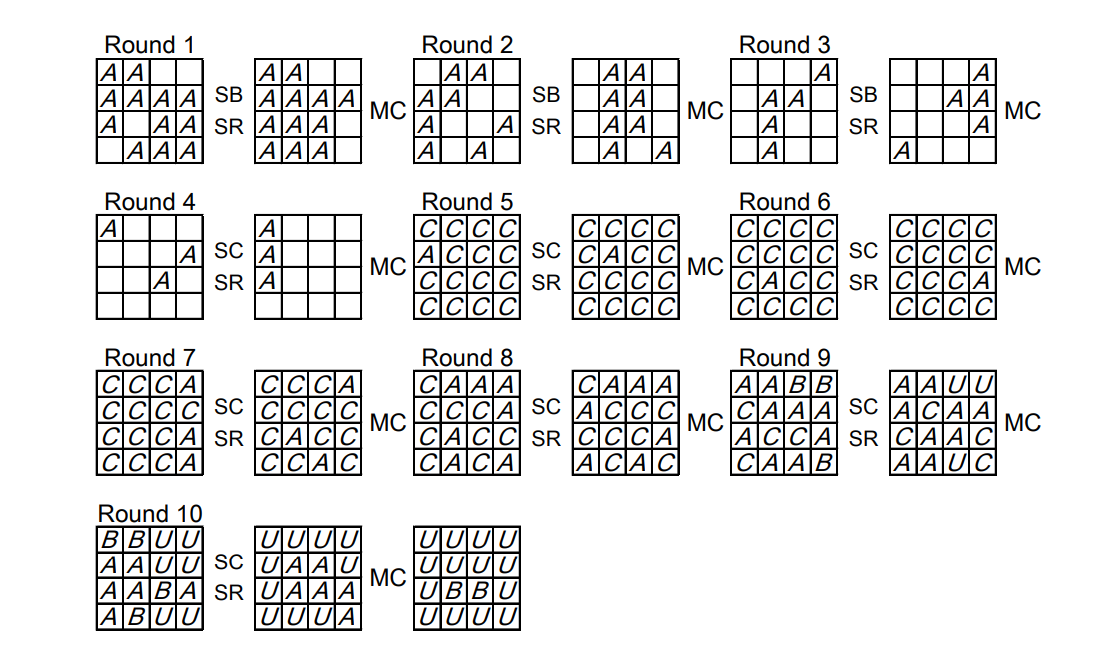
\includegraphics[width=12cm]{01.PNG}
	
\end{frame}

\begin{frame}{16 round Encryption}
	\centering
	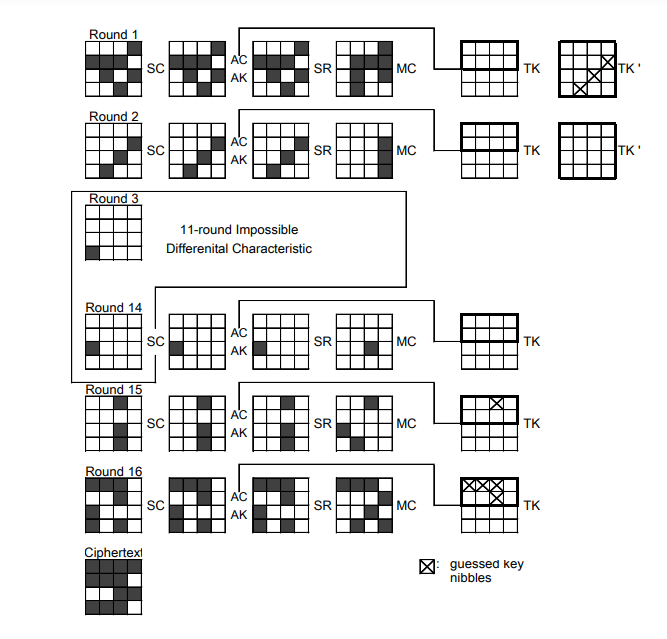
\includegraphics[width=8cm]{02.PNG}
	
\end{frame}
\begin{frame}{key recovery}
	
	\begin{itemize}[<+->]
		\item  prepares 
		$ 2^{12c}$
		plaintexts to form the integral distinguisher
		\item computes inverse MixColumns operation for each of the corresponding ciphertext,\\
		\item takes parity of the 4-cell values, This
		reduces the remaining text size to 2$^{8c}$
		.
		
		\item We do this 4 time and we reach 14-round to 10-round by backward track.
	\end{itemize}
\end{frame}
\begin{frame}{key recovery}
	\centering
	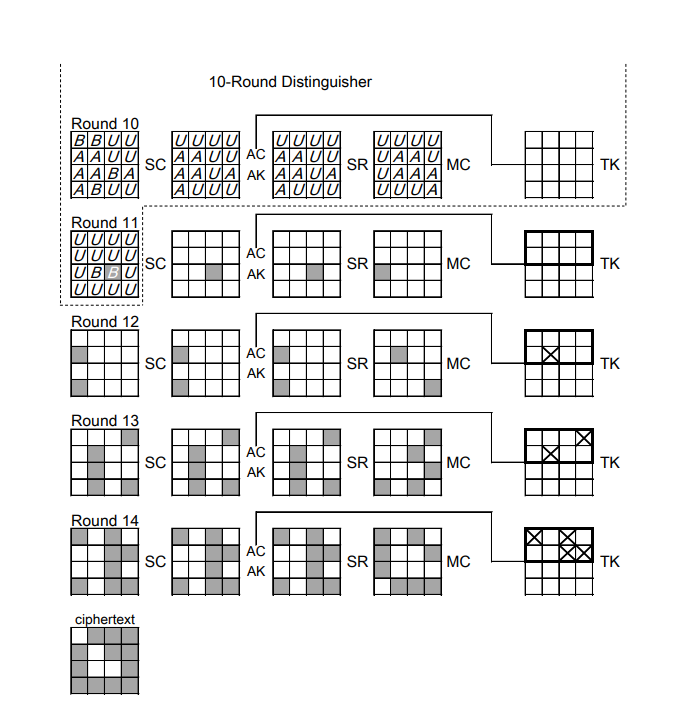
\includegraphics[width=8cm]{!!.PNG}
\end{frame}
\begin{frame}{Meet-In-The-Middle Attacks}
	
	With the help of this,Number of attack rounds can be calculate by considering the maximum length  of three features.Basically it work on SPN structure.
	\begin{itemize}[<+>]
		\item  Partial-Matching 
		\item Initial structure
		\item Splice-and-cut
		.
		
	\end{itemize}
	
\end{frame}
\begin{frame}{Meet-In-The-Middle Attacks}
	
	With the help of this,Number of attack rounds can be calculate by considering the maximum length  of three features.Basically it work on SPN structure.\\
	\begin{itemize}
		\item  Partial-Matching 
		\item Initial structure
		\item Splice-and-cut
		.
		
	\end{itemize}
	
\end{frame}
